\documentclass[a4paper]{article}
\usepackage{amsmath}
\usepackage{wasysym}
\usepackage{url}
\usepackage{tikz}
\usepackage{paralist}                        
\usepackage{xspace}  
\usepackage{qtree}             
\usetikzlibrary{calc}
\usetikzlibrary{fit}
\usetikzlibrary{arrows}
\usetikzlibrary{arrows,automata}
\usetikzlibrary{automata,positioning,arrows}
\usetikzlibrary{shapes}
\usetikzlibrary{shapes,backgrounds}
\usetikzlibrary{matrix}
\usetikzlibrary{chains,fit,shapes}

\DeclareMathOperator\caret{\raisebox{1ex}{$\scriptstyle\wedge$}}

\DeclareMathOperator{\DREG}{\mathsf{DREG}}
\DeclareMathOperator{\REG}{\mathsf{REG}}
\DeclareMathOperator{\DFA}{\mathsf{DFA}}
\DeclareMathOperator{\NFA}{\mathsf{NFA}}
\DeclareMathOperator{\eNFA}{\emptyword-\mathsf{NFA}}
\DeclareMathOperator{\DRX}{\mathsf{DRX}}
\DeclareMathOperator{\RX}{\mathsf{RX}}
\DeclareMathOperator{\fDRX}{\mathsf{DRX_{vsf}}}
\DeclareMathOperator{\fRX}{\mathsf{RX_{vsf}}}

\DeclareMathOperator{\TMFA}{\mathsf{TMFA}}
\DeclareMathOperator{\DTMFA}{\mathsf{DTMFA}}
\DeclareMathOperator{\fDTMFA}{\mathsf{DTMFA_{mcf}}}
\DeclareMathOperator{\fTMFA}{\mathsf{TMFA_{mcf}}}
\DeclareMathOperator{\DTMFAacc}{\mathsf{DTMFA^{acc}}}
\DeclareMathOperator{\DTMFArej}{\mathsf{DTMFA^{rej}}}
\DeclareMathOperator{\TMFAacc}{\mathsf{TMFA^{acc}}}
\DeclareMathOperator{\TMFArej}{\mathsf{TMFA^{rej}}}
\DeclareMathOperator{\fTMFArej}{\mathsf{TMFA^{rej}_{mcf}}}
\DeclareMathOperator{\fTMFAacc}{\mathsf{TMFA^{acc}_{mcf}}}
\DeclareMathOperator{\ellDTMFA}{\ell-\DTMFA}
\DeclareMathOperator{\MFA}{\mathsf{MFA}}

\DeclareMathOperator{\EXPTIME}{\mathsf{EXPTIME}}
\DeclareMathOperator{\PSPACE}{\mathsf{PSPACE}}
\DeclareMathOperator{\NPSPACE}{\mathsf{NPSPACE}}
\DeclareMathOperator{\NP}{\mathsf{NP}}
\DeclareMathOperator{\coNP}{\mathsf{coNP}}
%Markus' makro stuff

\DeclareMathOperator{\failstate}{\mathsf{[fail]}}
\DeclareMathOperator{\trapstate}{\mathsf{[trap]}}
\DeclareMathOperator{\open}{\mathtt{o}}
\DeclareMathOperator{\close}{\mathtt{c}}
\DeclareMathOperator{\reset}{\mathtt{r}}
\DeclareMathOperator{\unchanged}{\diamond}
\DeclareMathOperator{\opened}{\mathtt{O}}
\DeclareMathOperator{\closed}{\mathtt{C}}
\DeclareMathOperator{\prefequi}{\equiv}
\DeclareMathOperator{\nprefequi}{\not \equiv}
\newcommand{\ta}{\ensuremath{\mathtt{a}}}
\newcommand{\tb}{\ensuremath{\mathtt{b}}}
\newcommand{\tc}{\ensuremath{\mathtt{c}}}
\newcommand{\td}{\ensuremath{\mathtt{d}}}
\newcommand{\te}{\ensuremath{\mathtt{e}}}
\newcommand{\tf}{\ensuremath{\mathtt{f}}}
\newcommand{\tg}{\ensuremath{\mathtt{g}}}
\newcommand{\tth}{\ensuremath{\mathtt{h}}}
\newcommand{\tone}{\ensuremath{\mathtt{1}}}
\newcommand{\tzero}{\ensuremath{\mathtt{0}}}
\newcommand{\tRefX}{\ensuremath{\mathtt{\&x}}}
\newcommand{\tVarX}{\ensuremath{\mathtt{x}}}

% Dominik's macro stuff

\DeclareMathOperator{\df}{:=}
\DeclareMathOperator{\ror}{\vee} % currently using v as symbol for disjunction; other possibilities are + and |
\DeclareMathOperator*{\bigror}{\bigvee} % But: We need to have a good big version of it

\DeclareMathOperator*{\bigland}{\bigwedge} 
\DeclareMathOperator*{\biglor}{\bigvee} % biglor is used in logical formulas, bigror in regex 
\DeclareMathOperator{\sepA}{\#}
\DeclareMathOperator{\sepB}{\$}
\DeclareMathOperator{\sepC}{\cent}
\newcommand{\lang}{\mathcal{L}}
\newcommand{\langcl}{\mathcal{L}}
\newcommand{\emptyword}{\varepsilon}
\newcommand{\mdif}{\setminus}
\newcommand{\glush}{\mathcal{M}}
\DeclareMathOperator{\var}{\mathsf{var}}
%\newcommand{\bind}[2]{#1\{#2\}}
\newcommand{\bind}[2]{\langle#1\colon #2\rangle}
\newcommand{\rr}[1]{\&#1}
\newcommand{\refl}{\mathcal{R}}
\newcommand{\deref}{\mathcal{D}}
\DeclareMathOperator{\unmark}{\mathsf{unmark}}
%\newcommand{\vop}[1]{{\vdash_{#1}}}
%\newcommand{\vcl}[1]{{\dashv_{#1}}}
\newcommand{\vop}[1]{{[_{#1}}}
\newcommand{\vcl}[1]{{]_{#1}}}
\newcommand{\markpos}[1]{\tilde{#1}}
\newcommand{\mGamma}{\markpos{\Gamma}}
\newcommand{\mSigma}{\markpos{\Sigma}}
\newcommand{\mXi}{\markpos{\Xi}}

\newcommand{\ograph}[1]{G_{\markpos{#1}}}
\newcommand{\onodes}[1]{V_{\markpos{#1}}}
\newcommand{\oedges}[1]{E_{\markpos{#1}}}

\DeclareMathOperator{\src}{\mathsf{src}}
\DeclareMathOperator{\snk}{\mathsf{snk}}
\newcommand{\cheat}{\mathsf{ndet}}
\newcommand{\descitem}[1]{\textbf{\textsf{#1}}}
\newcommand{\ECreg}{\mathsf{EC^{reg}}}
\newcommand{\constr}{\mathsf{C}}
\newcommand{\const}[2]{\mathsf{C}_{#1}(#2)}
\newcommand{\hx}{\hat{x}}
\newcommand{\alpf}[1]{\alpha_{\mathsf{#1}}}
\newcommand{\Lcopy}{L_{\mathsf{copy}}}
\newcommand{\Lex}{L_{\mathsf{ex}}}
\newcommand{\clex}{\overline{\Lex}}
\DeclareMathOperator{\tin}{\mathsf{in}}
\DeclareMathOperator{\tout}{\mathsf{out}}
\newcommand{\alphasq}{\alpha_{\textsf{sq}}}
\newcommand{\fibword}{F_{\omega}}
\newcommand{\netvar}[1]{\mathsf{net}_{#1}}
\DeclareMathOperator{\gfirst}{\mathsf{first}}
\DeclareMathOperator{\gfollow}{\mathsf{follow}}
\DeclareMathOperator{\glast}{\mathsf{last}}
\newcommand{\alphar}{\alpha_{\refl}}
\newcommand{\betar}{\beta_{\refl}}
\newcommand{\gammar}{\gamma_{\refl}}
\newcommand{\glab}{\nu}
\DeclareMathOperator{\gmin}{\mathsf{min}}
\DeclareMathOperator{\splog}{\mathsf{SpLog}}


\begin{document}
% regular languages
~\newline
$\mathtt{L((a \cdot (b \ror c^+) \cdot a)^+)}$
\newline
$\mathtt{L(w~|~w~has~equal~number~of~a's) = L((b^* \cdot a \cdot b^* \cdot a \cdot b^*)^*)}$
\newline
$\mathtt{L(a^na^n) = L(a^{2n}) = L((a \cdot a)^*)}$

% non-regular languages
~\newline
$\mathtt{L(a^nb^n)}$
\newline
$\mathtt{L(a^nba^n)}$
\newline
$\mathtt{L(ww~|~w \in \Sigma^*, |\Sigma| > 1)}$
\newline

% regular languages with backreferences
~\newline
$\mathtt{L(a^nb^n) = L(\tVarX\{a^*\} \cdot b \cdot \tRefX)}$
\newline
$\mathtt{L(ww~|~w \in \Sigma^*, |\Sigma| > 1)} = L(\tVarX\{(a \ror b)^*\} \cdot \tRefX)$
	
%L(w | w has equal number of a’s)\newline
%Regex: (b* · a · b* · a · b*)*\newline
%L(anan) = L(a2*n) = L((a · a)*)\newline	
	\begin{center}
		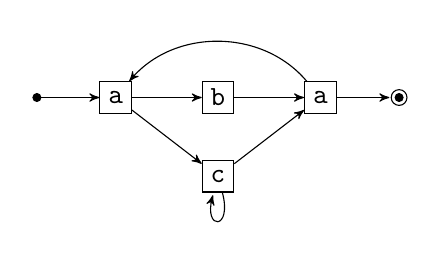
\begin{tikzpicture}[node distance=10mm,on grid,>=stealth',auto, 
		state/.style={rectangle,draw=black,inner sep=2pt,minimum size=4mm}]
		\node         (start)                 				{};
		\node[state]  (a1)     [right=of start] 				{$\ta$};
		\node[state]  (b)     [right=of a1, xshift=3mm]     	{$\tb$};
		\node[state]  (a2)     [right=of b,xshift=3mm] 				{$\ta$};
		\node[state]	(c)	[below=of b]		 	{$\tc$};
		
		\node 				(end)   [right=of a2]	   	{};
		
		\draw[fill=black] (start) circle (0.5mm);
		\draw[fill=black] (end) circle (0.5mm);
		\draw 						(end) circle (1mm);
		
		\path[->]
		(start.center) edge node[above, left=5pt,very near end,yshift=1mm] {} (a1)
		(a1) edge[] (b)
		(a1) edge[] (c)
		(c) edge[] (a2)
		(c) edge[loop below] (c)
		(b) edge[] (a2)
		(a2) edge[bend right=50] (a1)
		(a2) edge[] (end.west);
		\end{tikzpicture}
	\end{center}
	\vspace{-20pt}
	\begin{center}
		$(\ta \cdot (\tb\ror \tc^+) \cdot \ta)^+$
	\end{center}
	\vspace{5pt}


	\begin{center}
		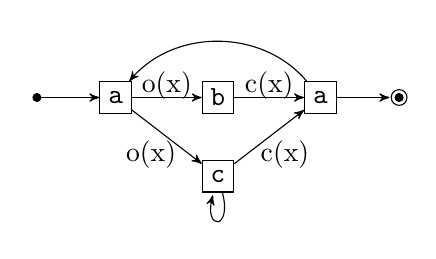
\begin{tikzpicture}[node distance=10mm,on grid,>=stealth',auto, 
		state/.style={rectangle,draw=black,inner sep=2pt,minimum size=4mm}]
		\node         (start)                 				{};
		\node[state]  (a1)     [right=of start] 				{$\ta$};
		\node[state]  (b)     [right=of a1, xshift=3mm]     	{$\tb$};
		\node[state]  (a2)     [right=of b,xshift=3mm] 				{$\ta$};
		\node[state]	(c)	[below=of b]		 	{$\tc$};
		
		\node 				(end)   [right=of a2]	   	{};
		
		\draw[fill=black] (start) circle (0.5mm);
		\draw[fill=black] (end) circle (0.5mm);
		\draw 						(end) circle (1mm);
		
		\path[->]
		(start.center) edge node[above, left=-5pt,very near end,yshift=1mm] {} (a1)
		(a1) edge[] node[yshift=-1.5mm]{o(x)} (b)
		(a1) edge[] node[below, xshift=-2mm, yshift=0.75mm]{o(x)} (c)
		(c) edge[] node[below, xshift=2mm, yshift=0.75mm]{c(x)} (a2)
		(c) edge[loop below] (c)
		(b) edge[] node[yshift=-1.5mm]{c(x)} (a2)
		(a2) edge[bend right=50] (a1)
		(a2) edge[] node[above, left=-5pt,very near end,yshift=1mm] {} (end.west);
		\end{tikzpicture}
	
	\end{center}
	\vspace{-20pt}
	\begin{center}
		$(\ta \cdot \tVarX\{(\tb\ror \tc^+)\} \cdot \ta)^+$
	\end{center}
	\vspace{5pt}


	\begin{center}
		
		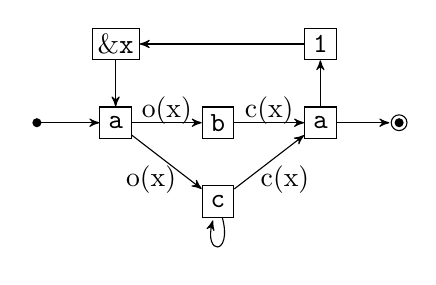
\begin{tikzpicture}[node distance=10mm,on grid,>=stealth',auto, 
		state/.style={rectangle,draw=black,inner sep=2pt,minimum size=4mm}]
		\node         (start)                 				{};
		
		\node[state]  (a1)     [right=of start] 				{$\ta$};
		\node[state]  (b)     [right=of a1, xshift=3mm]     	{$\tb$};
		\node[state]  (a2)     [right=of b,xshift=3mm] 				{$\ta$};
		\node[state]  (c)	[below=of b]		 	{$\tc$};
		\node[state]  (varX)	[above=of a1] {$\tRefX$};
		\node[state]  (one)     [above=of a2] {$\tone$};
		
		\node 				(end)   [right=of a2]	   	{};
		
		\draw[fill=black] (start) circle (0.5mm);
		\draw[fill=black] (end) circle (0.5mm);
		\draw 						(end) circle (1mm);
		
		\path[->]
		(start.center) edge node[above, left=-5pt,very near end,yshift=1mm] {} (a1)
		(a1) edge[] node[yshift=-1.5mm]{o(x)} (b)
		(a1) edge[] node[below, xshift=-2mm, yshift=0.75mm]{o(x)} (c)
		(c) edge[] node[below, xshift=2mm, yshift=0.75mm]{c(x)} (a2)
		(c) edge[loop below] (c)
		(b) edge[] node[yshift=-1.5mm]{c(x)} (a2)
		(a2) edge[] (one)
		(one) edge[] (varX)
		(varX) edge[] (a1)
		(a2) edge[] node[above, left=-5pt,very near end,yshift=1mm] {} (end.west);
		\end{tikzpicture}
		
	\end{center}
	\vspace{-20pt}
	\begin{center}
		$(\ta \cdot \tVarX\{(\tb\ror \tc^+)\} \cdot \ta) \cdot (\tone \cdot \tRefX \cdot \ta \cdot \tVarX\{(\tb\ror \tc^+)\} \cdot \ta)^*$
	\end{center}
	\vspace{5pt}

	\begin{center}
		
		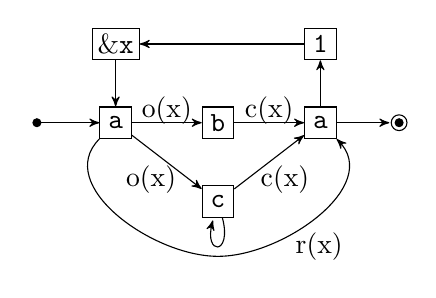
\begin{tikzpicture}[->,node distance=10mm,on grid,>=stealth',auto, 
		state/.style={rectangle,draw=black,inner sep=2pt,minimum size=4mm}]
		\node         (start)                 				{};
		
		\node[state]  (a1)     [right=of start] 				{$\ta$};
		\node[state]  (b)     [right=of a1, xshift=3mm]     	{$\tb$};
		\node[state]  (a2)     [right=of b,xshift=3mm] 				{$\ta$};
		\node[state]  (c)	[below=of b]		 	{$\tc$};
				\node[state]  (varX)	[above=of a1] {$\tRefX$};
		\node[state]  (one)     [above=of a2] {$\tone$};
		
		\node 				(end)   [right=of a2]	   	{};
		
		\draw[fill=black] (start) circle (0.5mm);
		\draw[fill=black] (end) circle (0.5mm);
		\draw 						(end) circle (1mm);
		
		\path[->]
		(start.center) edge node[above, left=-5pt,very near end,yshift=1mm] {} (a1)
		(a1) edge[] node[yshift=-1.5mm]{o(x)} (b)
		(a1) edge[] node[below, xshift=-2mm, yshift=0.75mm]{o(x)} (c)
		(c) edge[] node[below, xshift=2mm, yshift=0.75mm]{c(x)} (a2)
		(c) edge[loop below] (c)
		(b) edge[] node[yshift=-1.5mm]{c(x)} (a2)
		(a2) edge[] (one)
		(one) edge[] (varX)
		(varX) edge[] (a1)
		(a2) edge[] node[above, left=-5pt,very near end,yshift=1mm] {} (end.west);
		
		
		\draw (a1) to [out=225,in=180](current bounding box.south) to [out=0,in=315] node[below, yshift=-1mm]{r(x)} (a2);
		\end{tikzpicture}
	\end{center}
	\vspace{-20pt}
	\begin{center}
		$(\ta \cdot \tVarX\{(\tb\ror \tc^+ \ror \epsilon)\} \cdot \ta) \cdot (\tone \cdot \tRefX \cdot \ta \cdot \tVarX\{(\tb\ror \tc^+ \ror \epsilon )\} \cdot \ta)^*$
	\end{center}	

	\pagebreak
	
		\begin{center}
		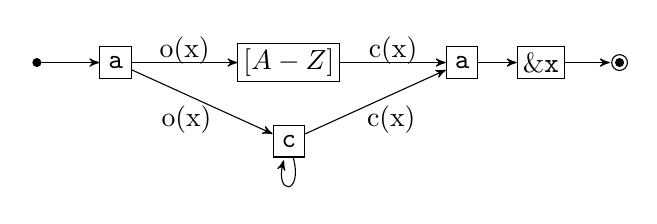
\begin{tikzpicture}[node distance=10mm,on grid,>=stealth',auto, 
		state/.style={rectangle,draw=black,inner sep=2pt,minimum size=4mm}]
		\node         (start)                 				{};
		\node[state]  (a1)     [right=of start] 				{$\ta$};
		\node[state]  (b)     [right=of a1, xshift=12mm]     	{$[A-Z]$};
		\node[state]  (a2)     [right=of b,xshift=12mm] 				{$\ta$};
		\node[state]	(c)	[below=of b]		 	{$\tc$};
		\node[state]  (refX) [right=of a2] {$\tRefX$};
		
		\node 				(end)   [right=of refX]	   	{};
		
		\draw[fill=black] (start) circle (0.5mm);
		\draw[fill=black] (end) circle (0.5mm);
		\draw 						(end) circle (1mm);
		
		\path[->]
		(start.center) edge node[above, left=-5pt,very near end,yshift=1mm] {} (a1)
		(a1) edge[] node[yshift=-1.5mm]{o(x)} (b)
		(a1) edge[] node[below, xshift=-2mm, yshift=0.75mm]{o(x)} (c)
		(c) edge[] node[below, xshift=2mm, yshift=0.75mm]{c(x)} (a2)
		(c) edge[loop below] (c)
		(b) edge[] node[yshift=-1.5mm]{c(x)} (a2)
		(a2) edge[] (refX)
		(refX) edge[] node[above, left=-5pt,very near end,yshift=1mm] {} (end.west);
		\end{tikzpicture}
		
	\end{center}
	\vspace{-20pt}
	\begin{center}
		$\ta \cdot \tVarX\{(\tb\ror \tc^+)\} \cdot \ta \cdot \tRefX$
	\end{center}

	\def\circle#1{\tikz\node[draw,circle]{#1};} 

	\Tree[.\circle{$\cdot$}
			[.\circle{$\cdot$}
				[.\circle{$\cdot$} 
				  [.\ta~ ]
				  [.\circle{x\{\}}
					  [.\circle{$\ror$} 
						  [.$[A-Z]$~ ]
						  [.\circle{$+$}
								[.\tc~ ]
						  ]
					  ]
					]
				 ]
				[.\ta~ ]
			]
			[.$\tRefX$ ]
		]

	\pagebreak
	
	
	\begin{center}
		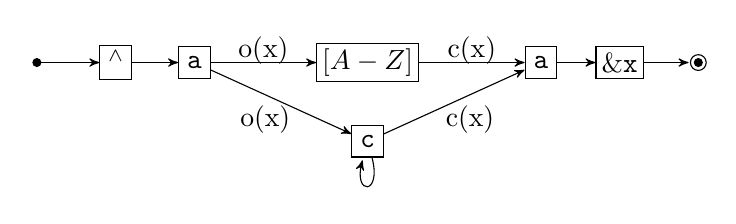
\begin{tikzpicture}[node distance=10mm,on grid,>=stealth',auto, 
		state/.style={rectangle,draw=black,inner sep=2pt,minimum size=4mm}]
		\node         (start)                 				{};
		\node[state]  (caret)  [right=of start] {$\caret$};
		\node[state]  (a1)     [right=of caret] 				{$\ta$};
		\node[state]  (b)     [right=of a1, xshift=12mm]     	{$[A-Z]$};
		\node[state]  (a2)     [right=of b,xshift=12mm] 				{$\ta$};
		\node[state]	(c)	[below=of b]		 	{$\tc$};
		\node[state]  (refX) [right=of a2] {$\tRefX$};
		
		\node 				(end)   [right=of refX]	   	{};
		
		\draw[fill=black] (start) circle (0.5mm);
		\draw[fill=black] (end) circle (0.5mm);
		\draw 						(end) circle (1mm);
		
		\path[->]
		(start.center) edge node[above, left=-5pt,very near end,yshift=1mm] {} (caret)
		(caret) edge (a1)
		(a1) edge[] node[yshift=-1.5mm]{o(x)} (b)
		(a1) edge[] node[below, xshift=-2mm, yshift=0.75mm]{o(x)} (c)
		(c) edge[] node[below, xshift=2mm, yshift=0.75mm]{c(x)} (a2)
		(c) edge[loop below] (c)
		(b) edge[] node[yshift=-1.5mm]{c(x)} (a2)
		(a2) edge[] (refX)
		(refX) edge[] node[above, left=-5pt,very near end,yshift=1mm] {} (end.west);
		\end{tikzpicture}
		
	\end{center}
	\vspace{-20pt}
	\begin{center}
		$\caret \cdot ~ \ta \cdot \tVarX\{([A-Z] \ror \tc^+)\} \cdot \ta \cdot \tRefX$
	\end{center}
	
	\def\circle#1{\tikz\node[draw,circle]{#1};} 
	
	\Tree[.\circle{$\cdot$}
	[.\circle{$\cdot$}
	[.\circle{$\cdot$} 
		[.\circle{$\cdot$}
			[.$\caret$ ]
		[.\ta~ ]
	]
	[.\circle{x\{\}}
	[.\circle{$\ror$} 
	[.$[A-Z]$~ ]
	[.\circle{$+$}
	[.\tc~ ]
	]
	]
	]
	]
	[.\ta~ ]
	]
	[.$\tRefX$ ]
	]
	
	\pagebreak
	
	\begin{center}
		\begin{tikzpicture}[node distance=10mm,on grid,>=stealth',auto, 
		state/.style={rectangle,draw=black,inner sep=2pt,minimum size=4mm}]
		\node         (start)                 				{};
		\node[state]  (caret)  [right=of start] {$\caret$};
		\node[state]  (a1)     [right=of caret] 				{$\ta$};
		\node[state]  (b)     [right=of a1, xshift=12mm]     	{$[A-Z]$};
		\node[state]  (a2)     [right=of b,xshift=12mm] 				{$\ta$};
		\node[state]	(c)	[below=of b]		 	{$\tc$};
		\node[state]  (refX) [right=of a2] {$\tRefX$};
		
		\node 				(end)   [right=of refX]	   	{};
		
		\draw[fill=black] (start) circle (0.5mm);
		\draw[fill=black] (end) circle (0.5mm);
		\draw 						(end) circle (1mm);
		
		\end{tikzpicture}
		
	\end{center}
	\vspace{-10pt}
	\begin{center}
		$\caret \cdot ~ \ta \cdot \tVarX\{([A-Z] \ror \tc^+)\} \cdot \ta \cdot \tRefX$
	\end{center}

	\pagebreak
	\begin{center}
		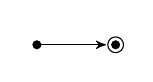
\begin{tikzpicture}[node distance=10mm,on grid,>=stealth',auto, 
		state/.style={rectangle,draw=black,inner sep=2pt,minimum size=4mm}]
		\node         (start)                 				{};		
		\node 				(end)   [right=of start]	   	{};
		
		\draw[fill=black] (start) circle (0.5mm);
		\draw[fill=black] (end) circle (0.5mm);
		\draw 						(end) circle (1mm);
		
		\path[->]
		(start.center) edge[] node[above, left=-5pt,very near end,yshift=1mm] {} (end.west);
		\end{tikzpicture}
		
	\end{center}
	\vspace{-20pt}
	\begin{center}
		$\epsilon$
	\end{center}

	~\newline
	
	\begin{center}
		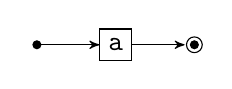
\begin{tikzpicture}[node distance=10mm,on grid,>=stealth',auto, 
		state/.style={rectangle,draw=black,inner sep=2pt,minimum size=4mm}]
		\node         (start)                 				{};
		\node[state]  (a1)     [right=of start] 				{$\ta$};		
		\node 				(end)   [right=of a1]	   	{};
		
		\draw[fill=black] (start) circle (0.5mm);
		\draw[fill=black] (end) circle (0.5mm);
		\draw 						(end) circle (1mm);
		
		\path[->]
		(start.center) edge node[above, left=-5pt,very near end,yshift=1mm] {} (a1)
		(a1) edge[] node[above, left=-5pt,very near end,yshift=1mm] {} (end.west);
		\end{tikzpicture}
		
	\end{center}
	\vspace{-20pt}
	\begin{center}
		$\ta$
	\end{center}

	~\newline
	
	\begin{center}
		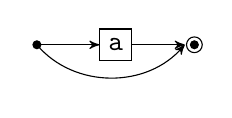
\begin{tikzpicture}[node distance=10mm,on grid,>=stealth',auto, 
		state/.style={rectangle,draw=black,inner sep=2pt,minimum size=4mm}]
		\node         (start)                 				{};
		\node[state]  (a1)     [right=of start] 				{$\ta$};		
		\node 				(end)   [right=of a1]	   	{};
		
		\draw[fill=black] (start) circle (0.5mm);
		\draw[fill=black] (end) circle (0.5mm);
		\draw 						(end) circle (1mm);
		
		\path[->]
		(start.center) edge node[above, left=-5pt,very near end,yshift=1mm] {} (a1)
		(start.center) edge[bend right=50] node[] {} (end.west)
		(a1) edge[] node[above, left=-5pt,very near end,yshift=1mm] {} (end.west);
		\end{tikzpicture}
		
	\end{center}
	\vspace{-20pt}
	\begin{center}
		$\ta \ror \epsilon$
	\end{center}
	~\newline

	\begin{center}
		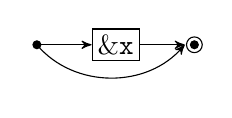
\begin{tikzpicture}[node distance=10mm,on grid,>=stealth',auto, 
		state/.style={rectangle,draw=black,inner sep=2pt,minimum size=4mm}]
		\node         (start)                 				{};
		\node[state]  (a1)     [right=of start] 				{$\tRefX$};		
		\node 				(end)   [right=of a1]	   	{};
		
		\draw[fill=black] (start) circle (0.5mm);
		\draw[fill=black] (end) circle (0.5mm);
		\draw 						(end) circle (1mm);
		
		\path[->]
		(start.center) edge node[above, left=-5pt,very near end,yshift=1mm] {} (a1)
		(start.center) edge[bend right=50] node[] {} (end.west)
		(a1) edge[] node[above, left=-5pt,very near end,yshift=1mm] {} (end.west);
		\end{tikzpicture}
		
	\end{center}
	\vspace{-20pt}
	\begin{center}
		$\tRefX \ror \epsilon$
	\end{center}

	~\newline
	
		
	\begin{center}
		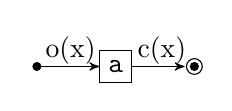
\begin{tikzpicture}[node distance=10mm,on grid,>=stealth',auto, 
		state/.style={rectangle,draw=black,inner sep=2pt,minimum size=4mm}]
		\node         (start)                 				{};
		\node[state]  (a1)     [right=of start] 				{$\ta$};		
		\node 				(end)   [right=of a1]	   	{};
		
		\draw[fill=black] (start) circle (0.5mm);
		\draw[fill=black] (end) circle (0.5mm);
		\draw 						(end) circle (1mm);
		
		\path[->]
		(start.center) edge node[above, left=-5pt,very near end,yshift=2mm] {o(x)} (a1)
		(a1) edge[] node[above, left=-5pt,very near end,xshift=0.5mm, yshift=2mm] {c(x)} (end.west);
		\end{tikzpicture}
		
	\end{center}
	\vspace{-10pt}
	\begin{center}
		$\tVarX\{\ta\}$
	\end{center}

	~\newline
	
	
	\begin{center}
		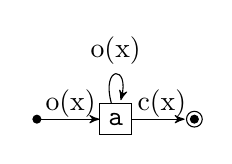
\begin{tikzpicture}[node distance=10mm,on grid,>=stealth',auto, 
		state/.style={rectangle,draw=black,inner sep=2pt,minimum size=4mm}]
		\node         (start)                 				{};
		\node[state]  (a1)     [right=of start] 				{$\ta$};		
		\node 				(end)   [right=of a1]	   	{};
		
		\draw[fill=black] (start) circle (0.5mm);
		\draw[fill=black] (end) circle (0.5mm);
		\draw 						(end) circle (1mm);
		
		\path[->]
		(start.center) edge node[above, left=-5pt,very near end,yshift=2mm] {o(x)} (a1)
		(a1) edge[loop above] node[above]{o(x)} (a1)
		(a1) edge[] node[above, left=-5pt,very near end,xshift=0.5mm, yshift=2mm] {c(x)} (end.west);
		\end{tikzpicture}
		
	\end{center}
	\vspace{-10pt}
	\begin{center}
		$\tVarX\{\ta\}^+$
	\end{center}

	~\newline
	
	
	\begin{center}
		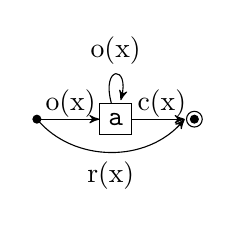
\begin{tikzpicture}[node distance=10mm,on grid,>=stealth',auto, 
		state/.style={rectangle,draw=black,inner sep=2pt,minimum size=4mm}]
		\node         (start)                 				{};
		\node[state]  (a1)     [right=of start] 				{$\ta$};		
		\node 				(end)   [right=of a1]	   	{};
		
		\draw[fill=black] (start) circle (0.5mm);
		\draw[fill=black] (end) circle (0.5mm);
		\draw 						(end) circle (1mm);
		
		\path[->]
		(start.center) edge node[above, left=-5pt,very near end,yshift=2mm] {o(x)} (a1)
		(a1) edge[loop above] node[above]{o(x)} (a1)
		(start.center) edge[bend right=50] node[below]{r(x)} (end.west)
		(a1) edge[] node[above, left=-5pt,very near end,xshift=0.5mm, yshift=2mm] {c(x)} (end.west);
		\end{tikzpicture}
		
	\end{center}
	\vspace{-10pt}
	\begin{center}
		$\tVarX\{\ta\}^*$
	\end{center}
	
	~\newline
	
	\begin{center}
		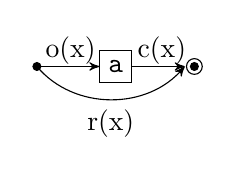
\begin{tikzpicture}[node distance=10mm,on grid,>=stealth',auto, 
		state/.style={rectangle,draw=black,inner sep=2pt,minimum size=4mm}]
		\node         (start)                 				{};
		\node[state]  (a1)     [right=of start] 				{$\ta$};		
		\node 				(end)   [right=of a1]	   	{};
		
		\draw[fill=black] (start) circle (0.5mm);
		\draw[fill=black] (end) circle (0.5mm);
		\draw 						(end) circle (1mm);
		
		\path[->]
		(start.center) edge node[above, left=-5pt,very near end,yshift=2mm] {o(x)} (a1)
		(start.center) edge[bend right=50] node[below]{r(x)} (end.west)
		(a1) edge[] node[above, left=-5pt,very near end,xshift=0.5mm, yshift=2mm] {c(x)} (end.west);
		\end{tikzpicture}
		
	\end{center}
	\vspace{-20pt}
	\begin{center}
		$\tVarX\{\ta \ror \epsilon\}$
	\end{center}

	~\newline
	
	\pagebreak

	\begin{center}
		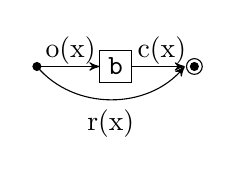
\begin{tikzpicture}[node distance=10mm,on grid,>=stealth',auto, 
		state/.style={rectangle,draw=black,inner sep=2pt,minimum size=4mm}]
		\node         (start)                 				{};
		\node[state]  (a1)     [right=of start] 				{$\tb$};		
		\node 				(end)   [right=of a1]	   	{};
		
		\draw[fill=black] (start) circle (0.5mm);
		\draw[fill=black] (end) circle (0.5mm);
		\draw 						(end) circle (1mm);
		
		\path[->]
		(start.center) edge node[above, left=-5pt,very near end,yshift=2mm] {o(x)} (a1)
		(start.center) edge[bend right=50] node[below]{r(x)} (end.west)
		(a1) edge[] node[above, left=-5pt,very near end,xshift=0.5mm, yshift=2mm] {c(x)} (end.west);
		\end{tikzpicture}
		
	\end{center}
	\vspace{-20pt}
	\begin{center}
		$\tVarX\{\tb \ror \epsilon\}$
	\end{center}

	~\newline

	\begin{center}
		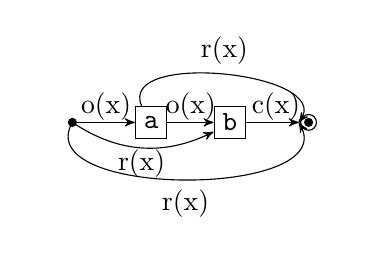
\begin{tikzpicture}[node distance=10mm,on grid,>=stealth',auto, 
		state/.style={rectangle,draw=black,inner sep=2pt,minimum size=4mm}]
		\node         (start)                 				{};
		\node[state]  (a1)     [right=of start] 				{$\ta$};
		\node[state]  (b)		[right=of a1]		{$\tb$};		
		\node 				(end)   [right=of b]	   	{};
		
		\draw[fill=black] (start) circle (0.5mm);
		\draw[fill=black] (end) circle (0.5mm);
		\draw 						(end) circle (1mm);
		
		\path[->]
		(start.center) edge node[above, left=-5pt,very near end,yshift=2mm] {o(x)} (a1)
		(start.center) edge[bend right=120] node[below]{r(x)} (end.west)
		(start.center) edge[bend right=30] node[below, yshift=1mm]{r(x)} (b)
		(a1) edge node[above, left=-5pt,very near end,xshift=0.5mm, yshift=2mm] {o(x)} (b)
		(a1) edge[bend left=120] node[above]{r(x)} (end.west)
		(b) edge[] node[above, left=-5pt,very near end,xshift=0.5mm, yshift=2mm] {c(x)} (end.west);
		\end{tikzpicture}
		
	\end{center}
	\vspace{-20pt}
	\begin{center}
		$\tVarX\{\ta \ror \epsilon\} \cdot \tVarX\{\tb \ror \epsilon\}$
	\end{center}


	\pagebreak

	~\newline	
	\begin{center}
		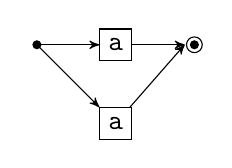
\begin{tikzpicture}[node distance=10mm,on grid,>=stealth',auto, 
		state/.style={rectangle,draw=black,inner sep=2pt,minimum size=4mm}]
		\node         (start)                 				{};
		\node[state]  (a1)     [right=of start] 				{$\ta$};	
		\node[state] (a2) [below=of a1]	{$\ta$};
		\node 				(end)   [right=of a1]	   	{};
		
		\draw[fill=black] (start) circle (0.5mm);
		\draw[fill=black] (end) circle (0.5mm);
		\draw 						(end) circle (1mm);
		
		\path[->]
		(start.center) edge node[above, left=-5pt,very near end,yshift=1mm] {} (a1)
		(start.center) edge[] node[] {} (a2)
		(a1) edge[] node[above, left=-5pt,very near end,yshift=1mm] {} (end.west)
		(a2) edge (end.west);
		\end{tikzpicture}
		
	\end{center}
	\vspace{-15pt}
	\begin{center}
		$\ta \ror \ta$
	\end{center}

	~\newline	
	\begin{center}
		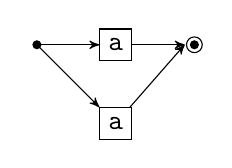
\begin{tikzpicture}[node distance=10mm,on grid,>=stealth',auto, 
		state/.style={rectangle,draw=black,inner sep=2pt,minimum size=4mm}]
		\node         (start)                 				{};
		\node[state]  (a1)     [right=of start] 				{$\ta$};	
		\node[state] (a2) [below=of a1]	{$\ta$};
		\node 				(end)   [right=of a1]	   	{};
		
		\draw[fill=black] (start) circle (0.5mm);
		\draw[fill=black] (end) circle (0.5mm);
		\draw 						(end) circle (1mm);
		
		\path[->]
		(start.center) edge node[above, left=-5pt,very near end,yshift=1mm] {} (a1)
		(start.center) edge[] node[] {} (a2)
		(a1) edge[] node[above, left=-5pt,very near end,yshift=1mm] {} (end.west)
		(a2) edge (end.west);
		\end{tikzpicture}
		
	\end{center}
	\vspace{-15pt}
	\begin{center}
		$\ta \ror \ta$
	\end{center}

	~\newline	
	\begin{center}
		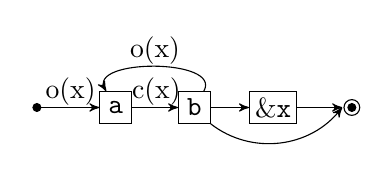
\begin{tikzpicture}[node distance=10mm,on grid,>=stealth',auto, 
		state/.style={rectangle,draw=black,inner sep=2pt,minimum size=4mm}]
		\node         (start)                 				{};
		\node[state]  (a1)     [right=of start] 				{$\ta$};	
		\node[state] (b) [right=of a1]	{$\tb$};
		\node[state] (refX) [right=of b] {$\tRefX$};
		\node 				(end)   [right=of refX]	   	{};
		
		\draw[fill=black] (start) circle (0.5mm);
		\draw[fill=black] (end) circle (0.5mm);
		\draw 						(end) circle (1mm);
		
		\path[->]
		(start.center) edge node[above, left=-5pt,very near end,yshift=2mm] {o(x)} (a1)
		(a1) edge[] node[above, left=-6.5pt,very near end,yshift=2mm] {c(x)} (b)
		(b) edge[bend right=120] node[above, yshift=-1mm] {o(x)} (a1)
		(b) edge[bend right=45] node[below] {} (end.west)
		(b) edge (refX)
		(refX) edge (end.west);
		\end{tikzpicture}
		
	\end{center}
	\vspace{-15pt}
	\begin{center}
		$(\tVarX \{ \ta \} \cdot \tb)^+ \cdot (\tRefX \ror \epsilon)$
	\end{center}

\end{document}
